%%%%%%%%%%%%%%%%%%%%%%%%%%%%%%%%%%%%%%%%%
% Technical Manual (Documentation Template)
% LaTeX Template
% Version 1.0 (05/01/2018)
%
% This template has been downloaded from:
% http://www.LaTeXTemplates.com
%
% Original author:
% Francisco Maria Calisto
%
% License:
% Apache License (Version 2.0)
%
% IMPORTANT NOTE:
% In addition to running BibTeX to compile the
% reference list from the .bib
% file, you will need to run MakeIndex to compile
% the index at the end of the document.
%
%%%%%%%%%%%%%%%%%%%%%%%%%%%%%%%%%%%%%%%%%

%---------------------------------------------------------------
%	PACKAGES AND OTHER DOCUMENT CONFIGURATIONS
%---------------------------------------------------------------

\documentclass{tufte-book} % Use the tufte-book class which in turn uses the tufte-common class

\usepackage{graphicx}
\graphicspath{ {graphics/} }

\usepackage{subfig}
\usepackage{listings}

% encoding
%--------------------------------------
\usepackage[utf8]{inputenc}
\usepackage[T1]{fontenc}
%--------------------------------------
 
% Portuguese-specific commands
%--------------------------------------
\usepackage[english]{babel}
%--------------------------------------

% Uncomment this line if you prefer colored hyperlinks
% (e.g., for onscreen viewing)
%--------------------------------------
\hypersetup{colorlinks}
%--------------------------------------

%%
% Book metadata
\title{Technical Manual\\(EN)}
\author[Technical Manual]{ISR \& INESC-ID}
\publisher{MIMBCD-UI}

%%
% If they're installed, use Bergamo and Chantilly from www.fontsite.com.
% They're clones of Bembo and Gill Sans, respectively.
%\IfFileExists{bergamo.sty}{\usepackage[osf]{bergamo}}{}% Bembo
%\IfFileExists{chantill.sty}{\usepackage{chantill}}{}% Gill Sans

%\usepackage{microtype}

%%
% Just some sample text
\usepackage{lipsum}

%%
% For nicely typeset tabular material
\usepackage{booktabs}

%%
% For graphics / images
\usepackage{graphicx}
\setkeys{Gin}{width=\linewidth,totalheight=\textheight,keepaspectratio}
\graphicspath{{graphics/}}

% The fancyvrb package lets us customize the formatting of verbatim
% environments.  We use a slightly smaller font.
\usepackage{fancyvrb}
\fvset{fontsize=\normalsize}

%%
% Prints argument within hanging parentheses (i.e., parentheses that take
% up no horizontal space).  Useful in tabular environments.
\newcommand{\hangp}[1]{\makebox[0pt][r]{(}#1\makebox[0pt][l]{)}}

%%
% Prints an asterisk that takes up no horizontal space.
% Useful in tabular environments.
\newcommand{\hangstar}{\makebox[0pt][l]{*}}

%%
% Prints a trailing space in a smart way.
\usepackage{xspace}

%%
% Some shortcuts for Tufte's book titles.  The lowercase commands will
% produce the initials of the book title in italics.  The all-caps commands
% will print out the full title of the book in italics.
\newcommand{\vdqi}{\textit{VDQI}\xspace}
\newcommand{\ei}{\textit{EI}\xspace}
\newcommand{\ve}{\textit{VE}\xspace}
\newcommand{\be}{\textit{BE}\xspace}
\newcommand{\VDQI}{\textit{The Visual Display of Quantitative Information}\xspace}
\newcommand{\EI}{\textit{Envisioning Information}\xspace}
\newcommand{\VE}{\textit{Visual Explanations}\xspace}
\newcommand{\BE}{\textit{Beautiful Evidence}\xspace}

\newcommand{\TL}{Tufte-\LaTeX\xspace}

% Prints the month name (e.g., January) and the year (e.g., 2008)
\newcommand{\monthyear}{%
  \ifcase\month\or January\or February\or March\or April\or May\or June\or
  July\or August\or September\or October\or November\or
  December\fi\space\number\year
}


% Prints an epigraph and speaker in sans serif, all-caps type.
\newcommand{\openepigraph}[2]{%
  %\sffamily\fontsize{14}{16}\selectfont
  \begin{fullwidth}
  \sffamily\large
  \begin{doublespace}
  \noindent\allcaps{#1}\\% epigraph
  \noindent\allcaps{#2}% author
  \end{doublespace}
  \end{fullwidth}
}

% Inserts a blank page
\newcommand{\blankpage}{\newpage\hbox{}\thispagestyle{empty}\newpage}

\usepackage{units}

% Typesets the font size, leading, and measure in the form of 10/12x26 pc.
\newcommand{\measure}[3]{#1/#2$\times$\unit[#3]{pc}}

% Macros for typesetting the documentation
\newcommand{\hlred}[1]{\textcolor{Maroon}{#1}}% prints in red
\newcommand{\hangleft}[1]{\makebox[0pt][r]{#1}}
\newcommand{\hairsp}{\hspace{1pt}}% hair space
\newcommand{\hquad}{\hskip0.5em\relax}% half quad space
\newcommand{\TODO}{\textcolor{red}{\bf TODO!}\xspace}
\newcommand{\ie}{\textit{i.\hairsp{}e.}\xspace}
\newcommand{\eg}{\textit{e.\hairsp{}g.}\xspace}
\newcommand{\na}{\quad--}% used in tables for N/A cells
\providecommand{\XeLaTeX}{X\lower.5ex\hbox{\kern-0.15em\reflectbox{E}}\kern-0.1em\LaTeX}
\newcommand{\tXeLaTeX}{\XeLaTeX\index{XeLaTeX@\protect\XeLaTeX}}
% \index{\texttt{\textbackslash xyz}@\hangleft{\texttt{\textbackslash}}\texttt{xyz}}
\newcommand{\tuftebs}{\symbol{'134}}% a backslash in tt type in OT1/T1
\newcommand{\doccmdnoindex}[2][]{\texttt{\tuftebs#2}}% command name -- adds backslash automatically (and doesn't add cmd to the index)
\newcommand{\doccmddef}[2][]{%
  \hlred{\texttt{\tuftebs#2}}\label{cmd:#2}%
  \ifthenelse{\isempty{#1}}%
    {% add the command to the index
      \index{#2 command@\protect\hangleft{\texttt{\tuftebs}}\texttt{#2}}% command name
    }%
    {% add the command and package to the index
      \index{#2 command@\protect\hangleft{\texttt{\tuftebs}}\texttt{#2} (\texttt{#1} package)}% command name
      \index{#1 package@\texttt{#1} package}\index{packages!#1@\texttt{#1}}% package name
    }%
}% command name -- adds backslash automatically
\newcommand{\doccmd}[2][]{%
  \texttt{\tuftebs#2}%
  \ifthenelse{\isempty{#1}}%
    {% add the command to the index
      \index{#2 command@\protect\hangleft{\texttt{\tuftebs}}\texttt{#2}}% command name
    }%
    {% add the command and package to the index
      \index{#2 command@\protect\hangleft{\texttt{\tuftebs}}\texttt{#2} (\texttt{#1} package)}% command name
      \index{#1 package@\texttt{#1} package}\index{packages!#1@\texttt{#1}}% package name
    }%
}% command name -- adds backslash automatically
\newcommand{\docopt}[1]{\ensuremath{\langle}\textrm{\textit{#1}}\ensuremath{\rangle}}% optional command argument
\newcommand{\docarg}[1]{\textrm{\textit{#1}}}% (required) command argument
\newenvironment{docspec}{\begin{quotation}\ttfamily\parskip0pt\parindent0pt\ignorespaces}{\end{quotation}}% command specification environment
\newcommand{\docenv}[1]{\texttt{#1}\index{#1 environment@\texttt{#1} environment}\index{environments!#1@\texttt{#1}}}% environment name
\newcommand{\docenvdef}[1]{\hlred{\texttt{#1}}\label{env:#1}\index{#1 environment@\texttt{#1} environment}\index{environments!#1@\texttt{#1}}}% environment name
\newcommand{\docpkg}[1]{\texttt{#1}\index{#1 package@\texttt{#1} package}\index{packages!#1@\texttt{#1}}}% package name
\newcommand{\doccls}[1]{\texttt{#1}}% document class name
\newcommand{\docclsopt}[1]{\texttt{#1}\index{#1 class option@\texttt{#1} class option}\index{class options!#1@\texttt{#1}}}% document class option name
\newcommand{\docclsoptdef}[1]{\hlred{\texttt{#1}}\label{clsopt:#1}\index{#1 class option@\texttt{#1} class option}\index{class options!#1@\texttt{#1}}}% document class option name defined
\newcommand{\docmsg}[2]{\bigskip\begin{fullwidth}\noindent\ttfamily#1\end{fullwidth}\medskip\par\noindent#2}
\newcommand{\docfilehook}[2]{\texttt{#1}\index{file hooks!#2}\index{#1@\texttt{#1}}}
\newcommand{\doccounter}[1]{\texttt{#1}\index{#1 counter@\texttt{#1} counter}}

% Generates the index
\usepackage{makeidx}
\makeindex

\begin{document}

% r.3 full title page
\maketitle

\let\cleardoublepage\clearpage

% r.5 contents
\tableofcontents

\let\cleardoublepage\clearpage

%%%%%%%%%%%%%%%%%%%%%%%%%%%%%%%%%%%%%%%%%%%%%%%%%%%%%%
% -------------------------------------------------- %
% -------------------------------------------------- %
% -------------------------------------------------- %
% -------------------------------------------------- %
%%%%%%%%%%%%%%%%%%%%%%%%%%%%%%%%%%%%%%%%%%%%%%%%%%%%%%

% r.9 introduction
\chapter{Intro}

This Technical Manual is intended to be used as a reference for the concepts and API's in MIMBCD-UI systems, more specifically, the \href{https://github.com/MIMBCD-UI/prototype-cornerstone}{\textit{prototype-cornerstone} repository}. If you are new to the system, we recommend that you start by reviewing the concepts below and then looking at the various examples to see how cornerstone is used. It is also useful to read the \href{https://github.com/MIMBCD-UI/master-dissertation}{Master Thesis of Francisco Maria Calisto\cite{mimbcd-ui_dissertation}} or a \href{https://dl.acm.org/citation.cfm?id=3134111&CFID=840856188&CFTOKEN=51535574}{related work\cite{Calisto:2017:TTM:3132272.3134111}}.

\hfill

\textbf{System Concepts}

\begin{itemize}
\item \textbf{Architecture}
\item \textbf{Image Processing}
\item \textbf{Viewport}
\end{itemize}

\hfill

%%%%%%%%%%%%%%%%%%%%%%%%%%%%%%%%%%%%%%%%%%%%%%%%%%%%%%
% -------------------------------------------------- %
% -------------------------------------------------- %
% -------------------------------------------------- %
% -------------------------------------------------- %
%%%%%%%%%%%%%%%%%%%%%%%%%%%%%%%%%%%%%%%%%%%%%%%%%%%%%%

% r.10 CHAPTER
\chapter{Architecture}

Some indiscriminate thoughts on the architecture where advantages on other libraries that where possible to minimize the amount of code to debug and maintain. In fact, no web framework shall be utilized such as \href{https://angularjs.org/}{AngularJS}, \href{http://backbonejs.org/}{Backbone}, \href{https://www.emberjs.com/}{EmberJS} or even \href{https://www.meteor.com/}{Meteor}. The \href{https://github.com/MIMBCD-UI/prototype-cornerstone}{\textit{prototype-cornerstone}} is focused on a layer lower than these frameworks and should not need them. Also, \href{https://github.com/MIMBCD-UI/prototype-cornerstone}{\textit{prototype-cornerstone}} should be useable with these frameworks though and possibly include adapters that make it easier to use in those frameworks.

Do not use libraries that force dependencies on users of the library. For example, it should be possible for an app that uses a different version of a library than cornerstone to work properly. Prefer small simple libraries to bigger ones. For instance, \href{https://jquery.com/}{jQuery} is too big. It should be possible to share the same library (as long as the version is supported by both).

Asynchronous APIs should leverage the deferred pattern to return promises that callers can use to properly handle success and failure conditions. The excellent \href{https://github.com/cujojs/when}{Cujo.js when library} has \href{https://github.com/cujojs/when/wiki}{great documentation} about this (and is used by our engine along with other cujo.js libraries such as \href{https://github.com/cujojs/rest}{REST} and \href{https://github.com/cujojs/curl}{CURL}). The API should present a simplified view of the medical imaging domain to make it easier for developers to work with.

The \href{https://github.com/MIMBCD-UI/prototype-cornerstone}{\textit{prototype-cornerstone}} can be framed into the diagram shown in the next image. More specifically, the implementation of the (i) \textbf{Client} service; accessed by the (ii) \textbf{MIMBCD-UI} services; and served by a (iii) \textbf{PACS} server (\href{https://www.orthanc-server.com/}{\textit{Orthanc}}). Part of the \href{https://www.dicomstandard.org/}{DICOM standard} must be accepted as a service of the \textbf{PACS} server type and must be the response answer of the \textbf{MIMBCD-UI} services, in order to determine the parameters. Additionally, the standard includes an exception with respect to several parameters.

We will first describe the (iii) \textbf{PACS} server (\href{https://www.orthanc-server.com/}{\textit{Orthanc}}), since we first upload the DICOM images through this system. Second, we will describe the (ii) \textbf{MIMBCD-UI} services, while it uses several libraries. Third, we will describe the (i) \textbf{Client}. The standard defines parameters in two variants; required and optional. If a \textbf{PACS} server (\href{https://www.orthanc-server.com/}{\textit{Orthanc}}) supports search by unique instance identifier, parameters of study and series are not necessary. The required parameters are those that identify unequivocally a DICOM object; the study identifiers, series and instance. All other parameters refer to modifications on the image or format of the data. This is the case of a server, which our system is implemented in, so the amount of parameters that should be treated and validated when doing searches, are reduced. The next image shows an UML sequence corresponding to with the execution of an \textbf{HTTP Request} on the \textbf{MIMBCD-UI} (WADO) services. The design of the service is explained below. Among these tools we can find support of Cornerstone \cite{arbelaiz2017volume} libraries. These libraries have in common being based in HTML5 and JavaScript so they allow the manipulation, display and access to DICOM object information completely in a web browser (\textbf{Client}).

\clearpage

%%%%%%%%%%%%%%%%%%%%%%%%%%%%%%%%%%%%%%%%%%%%%%%%%%%%%%

\begin{figure}[!hbt]
\begin{center}
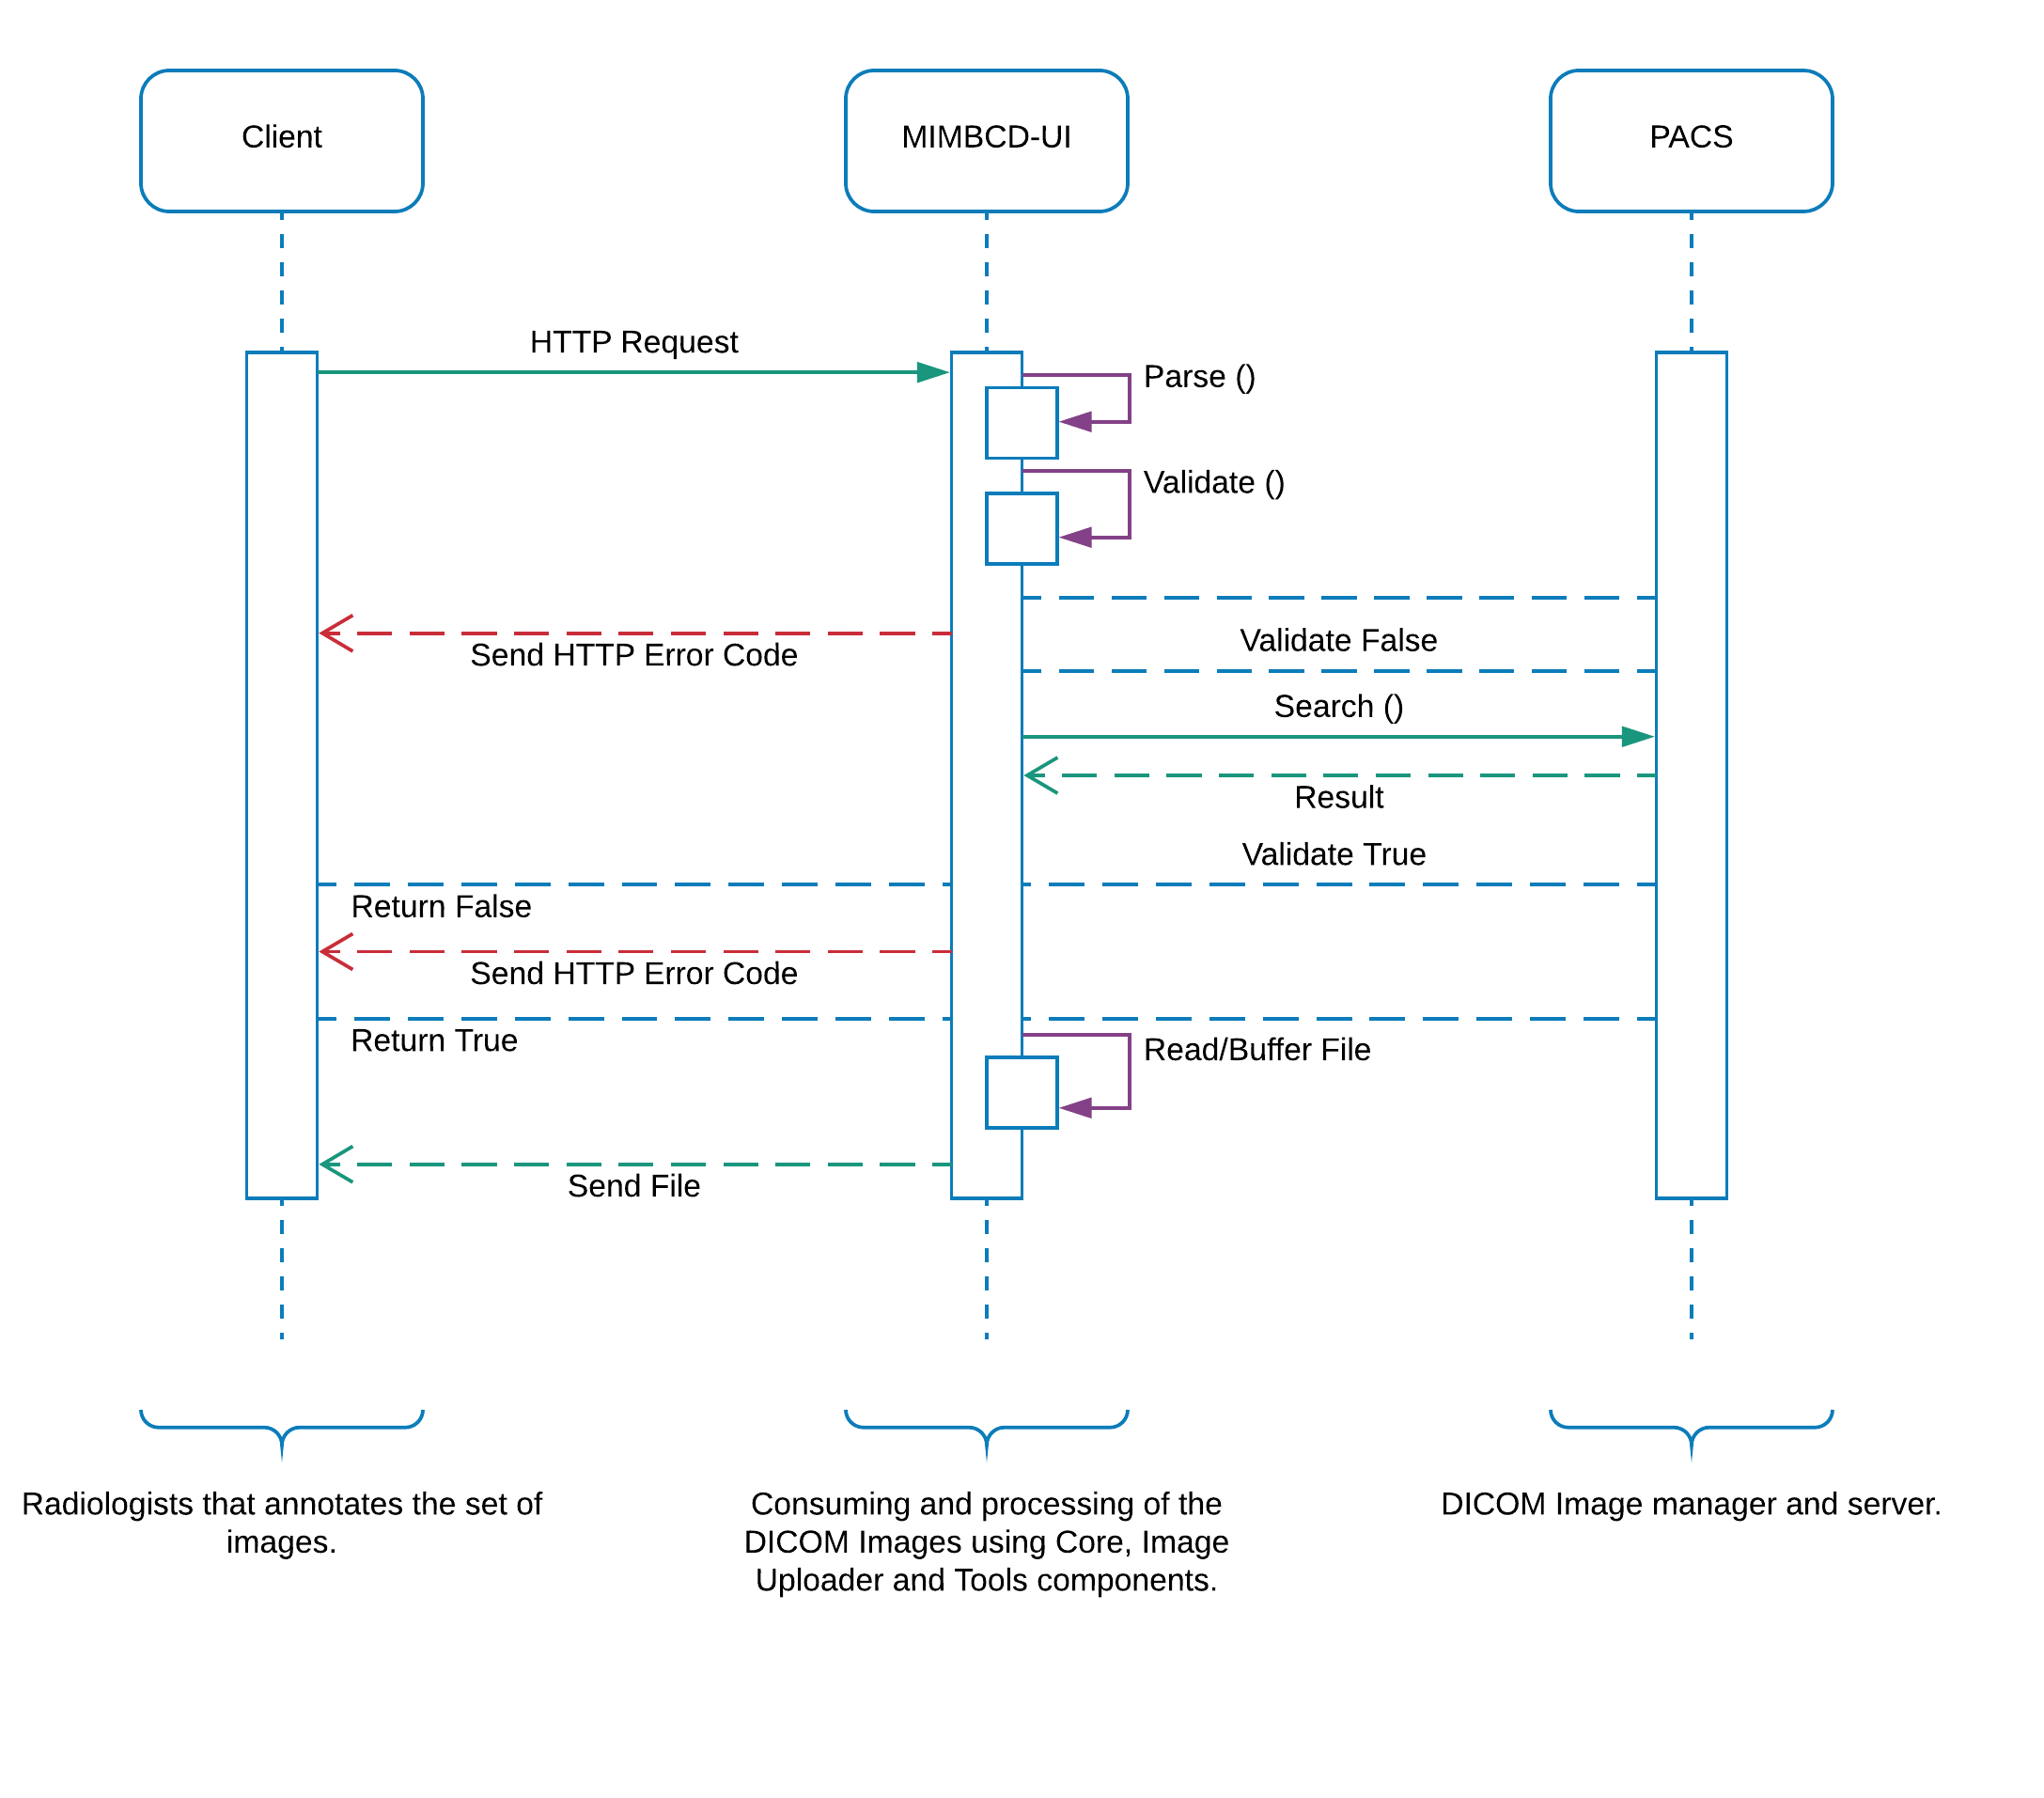
\includegraphics[width=\textwidth]{graphics/core_uml.png}
\end{center}
\end{figure}

%%%%%%%%%%%%%%%%%%%%%%%%%%%%%%%%%%%%%%%%%%%%%%%%%%%%%%

The ways of clarification, for the integration capacity are considered mainly two factors, if the tool allow us to easily configure it for an existing \textbf{PACS} and if the application type is compatible with an AWS server like an EC2. This last aspect is only considered for the convenience that the \textbf{PACS} services used with \textbf{MIMBCD-UI} System services are deployed on an AWS server. As a research of this study it was decided to explore the \href{https://github.com/cornerstonejs}{Cornerstone libraries} to create a web-based DICOM viewer. While it is a solution that requires greater implementation effort than those studied, which offer a fully functional image viewer, it is a basis for with a multimodality of medical imaging capabilities. \href{https://github.com/cornerstonejs}{Cornerstone} is a JavaScript library designed to show medical images in a web environment by doing use of the HTML5 Canvas element. \href{https://github.com/cornerstonejs/cornerstone}{Cornerstone Core} is not meant to be a complete application itself, but instead a component that can be used as part of larger more complex applications. The \textbf{MIMBCD-UI} System services are an example of using the various \href{https://github.com/cornerstonejs}{Cornerstone libraries} to build a simple study viewer.

\clearpage

\href{https://github.com/cornerstonejs/cornerstone}{Cornerstone Core} is agnostic to the actual container used to store image pixels and to transport mechanisms used to get the image data. As a matter of fact, \href{https://github.com/cornerstonejs/cornerstone}{Cornerstone Core} itself has no ability to read/parse or load images and instead depends on one or more \textit{ImageLoader} and \textit{dicomParser} (\textbf{Validate ()} and \textbf{Parse ()} from the last figure to function. The goal here is to avoid constraining developers to work within a single container and transport since images are stored in a variety of formats (e.g. DICOM). By providing flexibility with respect to the container and transport, the highest performance image display may be obtained as no conversion to an alternate container or transport is required. It is hoped that developers feel empowered to load images from any type of image container using any kind of transport. See the \href{https://github.com/cornerstonejs/cornerstoneWADOImageLoader}{\textit{CornerstoneWADOImageLoader}} repository for an example of a \href{https://github.com/cornerstonejs/cornerstone/wiki/ImageLoader}{DICOM WADO based Image Loader}.

\hfill

The \href{https://github.com/MIMBCD-UI/prototype-cornerstone}{\textit{prototype-cornerstone}} often have associated data with it. Several tools might need to keep track of the starting and ending \href{https://github.com/cornerstonejs/cornerstone/wiki/Pixel-Coordinate-System}{pixel coordinates} of the length measurement and which \href{https://github.com/cornerstonejs/cornerstone/wiki/ImageIds}{ImageId} it is associated with. The cornerstone tools library addresses this by providing the following API functions to work with tool specific data.

\hfill

The \textit{addToolState} API call is used to add tool specific data to the tool data context associated with an \href{https://github.com/cornerstonejs/cornerstone/wiki/enabled-element}{enabled element}.

\hfill

\begin{lstlisting}
function addToolState(element, toolType, data)
\end{lstlisting}

\hfill

The \textit{getToolState} API call is used to get tool specific data for the tool data context associated with an enabled element.

\hfill

\begin{lstlisting}
function getToolState(element, toolType)
\end{lstlisting}

\hfill

To better understand and to have more details about the hereby information, just follow the \href{https://github.com/cornerstonejs/cornerstoneTools/wiki/DataManagement}{\textit{DataManagement}} wiki.

%%%%%%%%%%%%%%%%%%%%%%%%%%%%%%%%%%%%%%%%%%%%%%%%%%%%%%
% -------------------------------------------------- %
% -------------------------------------------------- %
% -------------------------------------------------- %
% -------------------------------------------------- %
%%%%%%%%%%%%%%%%%%%%%%%%%%%%%%%%%%%%%%%%%%%%%%%%%%%%%%

% r.10 CHAPTER
\chapter{Image Processing}

Communication between devices using the \href{https://www.ncbi.nlm.nih.gov/pmc/articles/PMC61235/}{DICOM network protocol} is done via \href{https://en.wikipedia.org/wiki/Transmission_Control_Protocol}{TCP} and \href{https://en.wikipedia.org/wiki/IP_address}{IP}. To establish a connection, devices or applications negotiate who is the client and who is the server and establish an association. Once associated, orders can be sent to copy, save, delete and move \href{http://isdis.net/wp-content/uploads/2015/12/caffery_objects_IM.pdf}{DICOM objects}. \href{http://isdis.net/wp-content/uploads/2015/12/caffery_objects_IM.pdf}{DICOM objects} are not limited to image data, it contains a data structure with a large amount of meta information. Each element within a \href{http://isdis.net/wp-content/uploads/2015/12/caffery_objects_IM.pdf}{DICOM object} is classified according to a dictionary of identifying tags uniquely a data field. Among these labels, very numerous, there are fields that point to the patient's data (name, date of birth), data of the image and to what study and series the object belongs. To clarify what a series in \href{http://isdis.net/wp-content/uploads/2015/12/caffery_objects_IM.pdf}{DICOM} is, we must refer to the hierarchy, present in the following diagram. In this standard one patient has multiple studies, one study has multiple series and a series has multiple instances (images, \href{http://isdis.net/wp-content/uploads/2015/12/caffery_objects_IM.pdf}{DICOM objects}).

%%%%%%%%%%%%%%%%%%%%%%%%%%%%%%%%%%%%%%%%%%%%%%%%%%%%%%

\hfill

\begin{figure}[!hbt]
\begin{center}
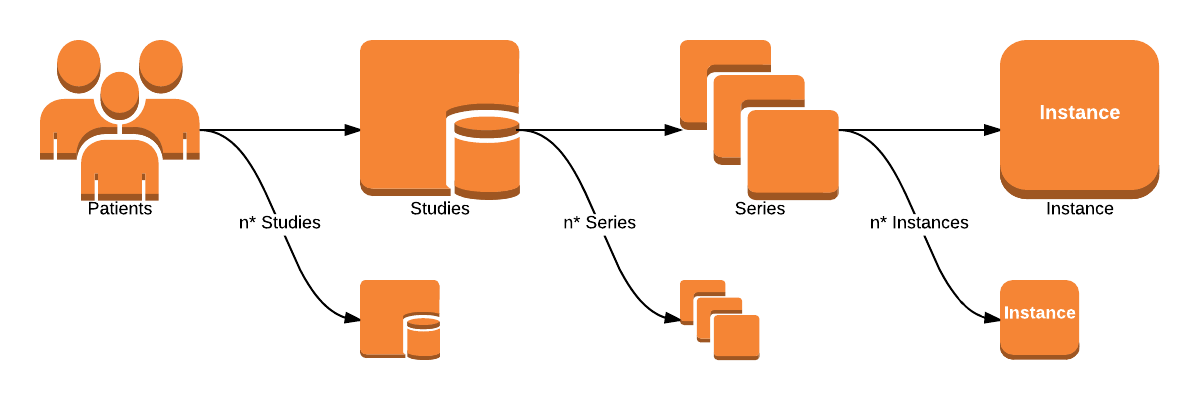
\includegraphics[width=\textwidth]{graphics/dicom_objects.png}
\end{center}
\end{figure}

\hfill

%%%%%%%%%%%%%%%%%%%%%%%%%%%%%%%%%%%%%%%%%%%%%%%%%%%%%%

One of the main goals of the standard is that \href{http://isdis.net/wp-content/uploads/2015/12/caffery_objects_IM.pdf}{DICOM objects} can be uniquely identified. On a \href{http://isdis.net/wp-content/uploads/2015/12/caffery_objects_IM.pdf}{DICOM objects}, the patient's data, the image and other data that relate to one object to the other (such as \textbf{Series} and \textbf{Studies}) are unequivocally bound. A part of the standard describes how requests and responses should be in a web service that serves \href{http://isdis.net/wp-content/uploads/2015/12/caffery_objects_IM.pdf}{DICOM objects} and throughout its evolution has incorporated definitions for web services and \href{https://en.wikipedia.org/wiki/Representational_state_transfer}{RESTful API}. This part of the standard is of particular interest to the \href{https://github.com/MIMBCD-UI/prototype-cornerstone}{\textit{prototype-cornerstone}} since the goal of allowing access to objects like \href{http://isdis.net/wp-content/uploads/2015/12/caffery_objects_IM.pdf}{DICOM objects} via an UI can be ideally developed by implementing a service that complies with the specifications of the standard.

\clearpage

Our \href{https://github.com/MIMBCD-UI/prototype-cornerstone}{\textit{prototype-cornerstone}} has an Image Loader for \href{http://www.web3.lu/dicom-standard/}{DICOM P10} instances over \href{http://dicom.nema.org/dicom/2013/output/chtml/part18/sect_6.3.html}{HTTP (WADO-URI)}. Nevertheless, it can also be also be pair with a \href{http://dicom.nema.org/medical/dicom/current/output/html/part18.html}{DICOMWeb (WADO-RS)}. We are using our \href{https://github.com/MIMBCD-UI/prototype-cornerstone}{\textit{prototype-cornerstone}} integrated with \href{http://dicom.nema.org/dicom/2013/output/chtml/part18/sect_6.3.html}{WADO-URI servers}, a \href{https://en.wikipedia.org/wiki/Web_API}{HTTP based server} that returns \href{http://www.web3.lu/dicom-standard/}{DICOM P10} instances called \href{https://www.orthanc-server.com/}{Orthanc Server}. The following Figure shows how we obtained each instance information related to the patients to be read by the \textbf{MIMBCD-UI} System on the \href{https://github.com/MIMBCD-UI/prototype-cornerstone}{\textit{prototype-cornerstone}} repository.

%%%%%%%%%%%%%%%%%%%%%%%%%%%%%%%%%%%%%%%%%%%%%%%%%%%%%%

\hfill

\begin{figure}[!hbt]
\begin{center}
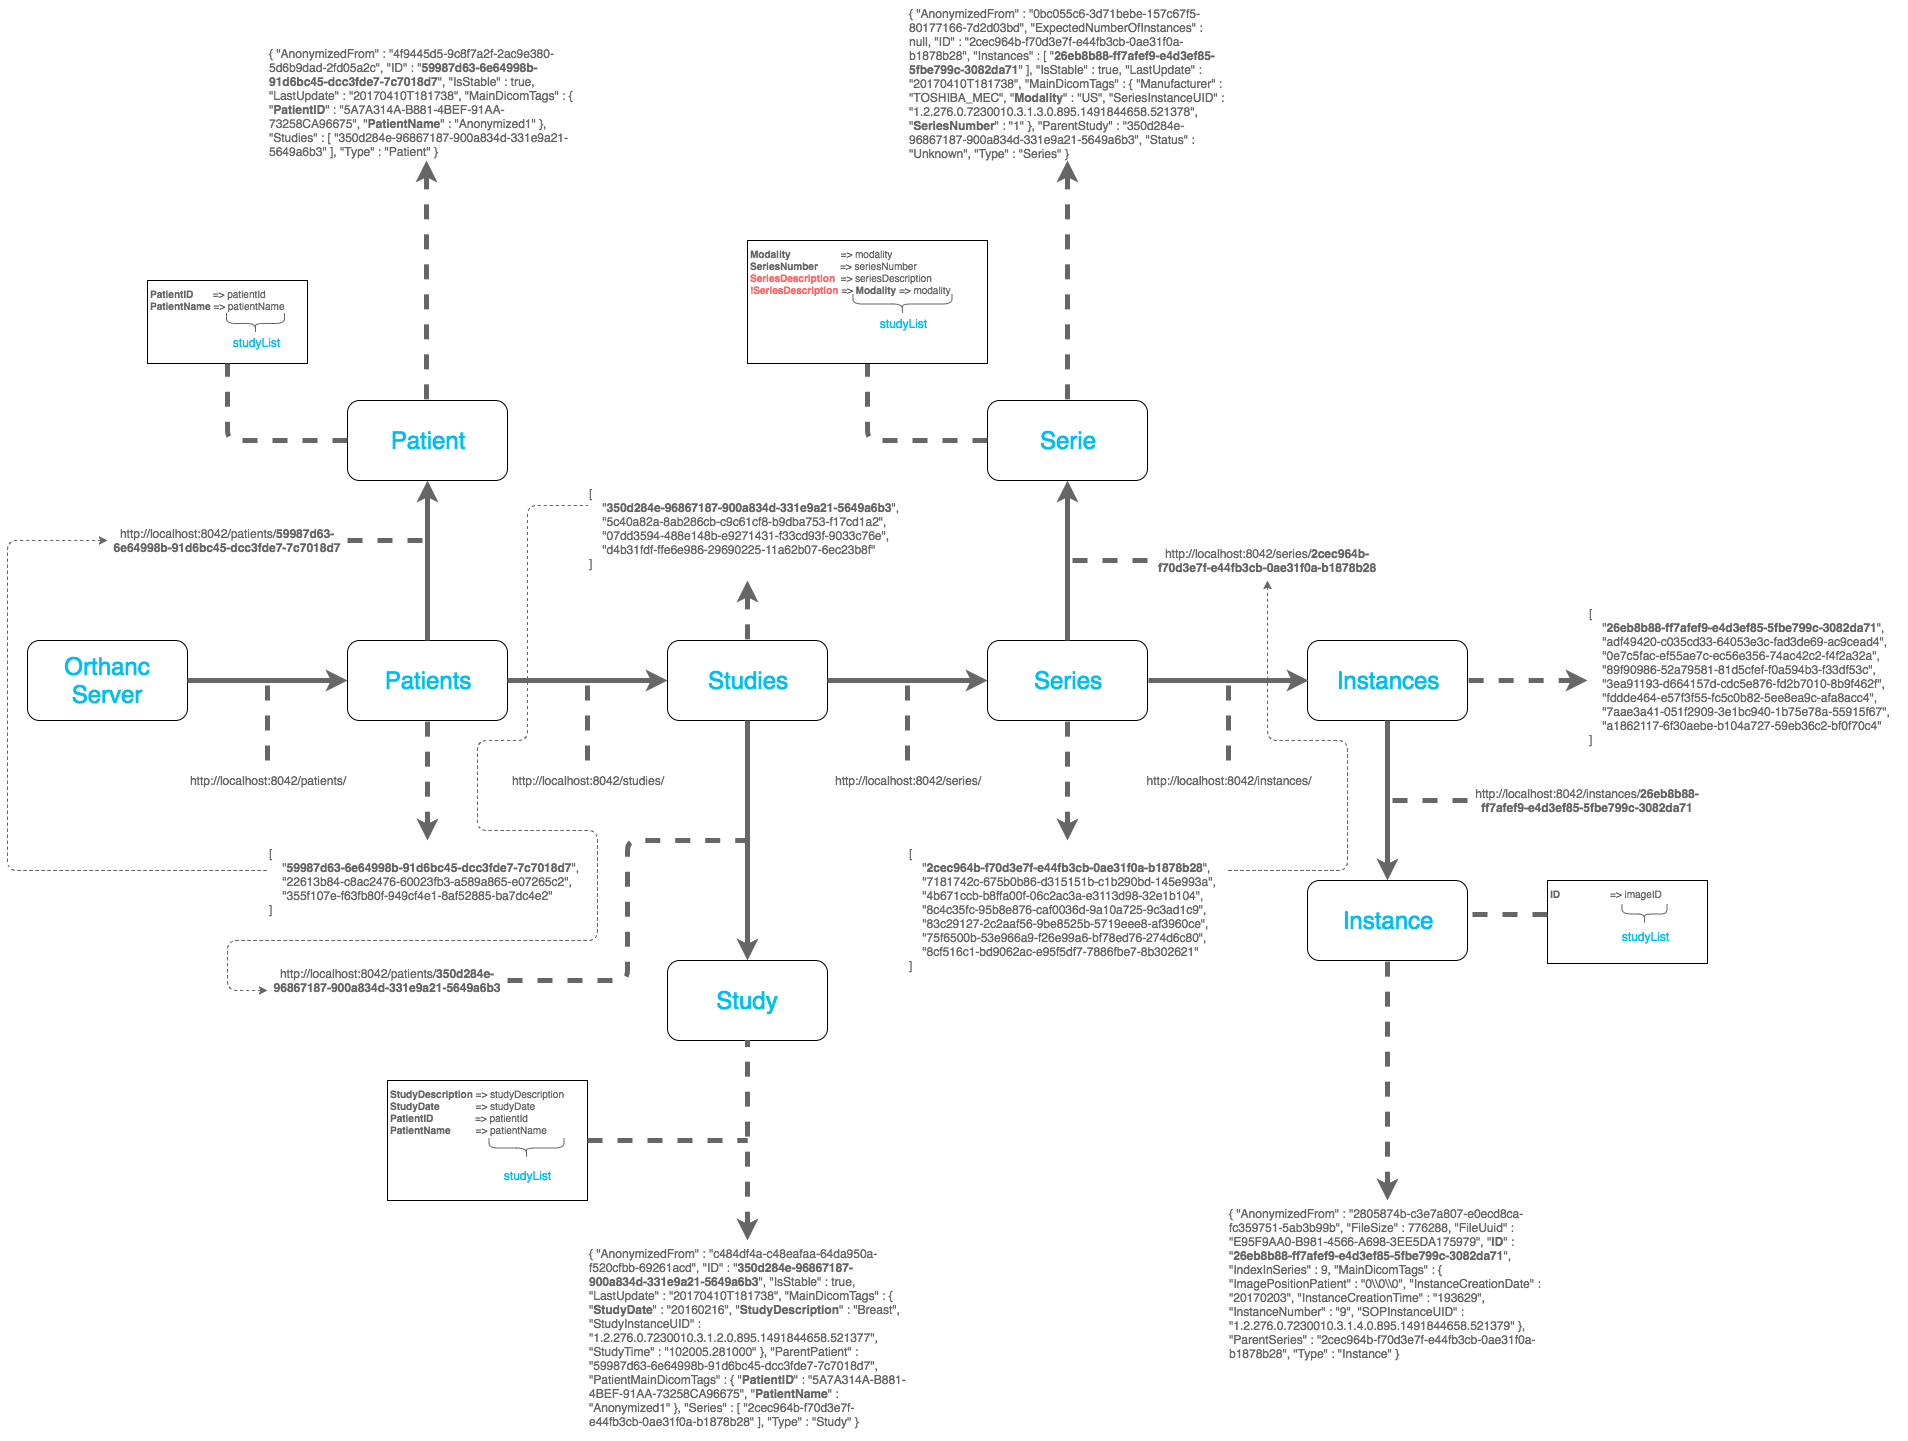
\includegraphics[width=\textwidth]{graphics/orthanc_example.png}
\end{center}
\end{figure}

\hfill

%%%%%%%%%%%%%%%%%%%%%%%%%%%%%%%%%%%%%%%%%%%%%%%%%%%%%%

While \href{https://www.orthanc-server.com/}{Orthanc Servers} are therefore built-in \href{https://en.wikipedia.org/wiki/Representational_state_transfer}{RESTful API}, it can be used to drive \href{https://www.orthanc-server.com/}{Orthanc} from external application, as shown on the above figure. That way \href{https://www.orthanc-server.com/}{Orthanc} is independent of the programming language that is used to develop other applications, in our case, for our \href{https://github.com/MIMBCD-UI/prototype-cornerstone}{\textit{prototype-cornerstone}}.

To use \href{https://www.orthanc-server.com/}{Orthanc} just open the \href{http://book.orthanc-server.com/users/cookbook.html}{Orthanc Explorer}. The embedded administrative interface of \href{https://www.orthanc-server.com/}{Orthanc}, with a browser. It entirely resorts to the \href{https://en.wikipedia.org/wiki/Representational_state_transfer}{RESTful API} for all its features. So that, anything that can be done through \href{http://book.orthanc-server.com/users/cookbook.html}{Orthanc Explorer}, can also be done trough \href{http://book.orthanc-server.com/users/rest.html}{REST queries}.

\clearpage

%----------------------------------------------------%

\textbf{Patients}

\hfill

The \href{https://www.orthanc-server.com/}{Orthanc Server} structures the stored \href{http://book.orthanc-server.com/users/rest.html#sending-dicom-images}{DICOM resources} using the \textbf{Patient} model of the \href{https://www.dicomstandard.org/current/}{DICOM standard}. Each \href{http://book.orthanc-server.com/users/rest.html#sending-dicom-images}{DICOM resources} is associated with an unique identifier:

\begin{lstlisting}
http://localhost:8042/patients/
\end{lstlisting}

\hfill

Here is how you would list of \textbf{Patients} for the DICOM resources that are stored in your local \href{http://book.orthanc-server.com/faq/rest-samples.html}{Orthanc instance}:

\begin{lstlisting}
[
   "59987d63-6e64998b-91d6bc45-dcc3fde7-7c7018d7",
   "22613b84-c8ac2476-60023fb3-a589a865-e07265c2",
   "355f107e-f63fb80f-949cf4e1-8af52885-ba7dc4e2"
]
\end{lstlisting}

\hfill

To access a single resource, add its identifier to the \href{https://en.wikipedia.org/wiki/Uniform_resource_identifier}{URI}. You would for instance retrieve the main information about one \textbf{Patient} as follows:

\begin{lstlisting}
http://localhost:8042/patients/59987d63-6e64998b-91d6bc45-dcc3fde7-7c7018d7
\end{lstlisting}

\hfill

Here is a possible answer from \href{https://www.orthanc-server.com/}{Orthanc}:

\begin{lstlisting}
{
   "AnonymizedFrom" : "4f9445d5-9c8f7a2f-2ac9e380-5d6b9dad-2fd05a2c",
   "ID" : "59987d63-6e64998b-91d6bc45-dcc3fde7-7c7018d7",
   "IsStable" : true,
   "LastUpdate" : "20170410T181738",
   "MainDicomTags" : {
      "PatientID" : "5A7A314A-B881-4BEF-91AA-73258CA96675",
      "PatientName" : "Anonymized1"
   },
   "Studies" : [ "350d284e-96867187-900a834d-331e9a21-5649a6b3" ],
   "Type" : "Patient"
}
\end{lstlisting}

%----------------------------------------------------%

\clearpage

%----------------------------------------------------%

\textbf{Studies}

\hfill

The \href{https://www.orthanc-server.com/}{Orthanc Server} structures the stored \href{http://book.orthanc-server.com/users/rest.html#sending-dicom-images}{DICOM resources} using the \textbf{Study} model of the \href{https://www.dicomstandard.org/current/}{DICOM standard}. Each \href{http://book.orthanc-server.com/users/rest.html#sending-dicom-images}{DICOM resources} is associated with an unique identifier:

\begin{lstlisting}
http://localhost:8042/studies/
\end{lstlisting}

\hfill

The field \textbf{Studies} list all the \href{http://book.orthanc-server.com/users/rest.html#sending-dicom-images}{DICOM studies} that are associated with the \textbf{Patient}. So, considering the \textbf{Patient} above, we would go down in her \href{http://book.orthanc-server.com/users/rest.html#sending-dicom-images}{DICOM} hierarchy as follows:

\begin{lstlisting}
[
   "350d284e-96867187-900a834d-331e9a21-5649a6b3",
   "5c40a82a-8ab286cb-c9c61cf8-b9dba753-f17cd1a2",
   "07dd3594-488e148b-e9271431-f33cd93f-9033c76e",
   "d4b31fdf-ffe6e986-29690225-11a62b07-6ec23b8f"
]
\end{lstlisting}

\hfill

To access a single resource, add its identifier to the \href{https://en.wikipedia.org/wiki/Uniform_resource_identifier}{URI}. You would for instance retrieve the main information about one \textbf{Study} as follows:

\begin{lstlisting}
http://localhost:8042/studies/350d284e-96867187-900a834d-331e9a21-5649a6b3
\end{lstlisting}

\hfill

Here is a possible answer from \href{https://www.orthanc-server.com/}{Orthanc}:

\begin{lstlisting}
{
   "AnonymizedFrom" : "c484df4a-c48eafaa-64da950a-f520cfbb-69261acd",
   "ID" : "350d284e-96867187-900a834d-331e9a21-5649a6b3",
   "IsStable" : true,
   "LastUpdate" : "20170410T181738",
   "MainDicomTags" : {
      "StudyDate" : "20160216",
      "StudyDescription" : "Breast",
      "StudyInstanceUID" : "1.2.276.0.7230010.3.1.2.0.895.1491844658.521377",
      "StudyTime" : "102005.281000"
   },
   "ParentPatient" : "59987d63-6e64998b-91d6bc45-dcc3fde7-7c7018d7",
   "PatientMainDicomTags" : {
      "PatientID" : "5A7A314A-B881-4BEF-91AA-73258CA96675",
      "PatientName" : "Anonymized1"
   },
   "Series" : [ "2cec964b-f70d3e7f-e44fb3cb-0ae31f0a-b1878b28" ],
   "Type" : "Study"
}
\end{lstlisting}

%----------------------------------------------------%

\clearpage

%----------------------------------------------------%

\textbf{Series}

\hfill

The \href{https://www.orthanc-server.com/}{Orthanc Server} structures the stored \href{http://book.orthanc-server.com/users/rest.html#sending-dicom-images}{DICOM resources} using the \textbf{Serie} model of the \href{https://www.dicomstandard.org/current/}{DICOM standard}. Each \href{http://book.orthanc-server.com/users/rest.html#sending-dicom-images}{DICOM resources} is associated with an unique identifier:

\begin{lstlisting}
http://localhost:8042/series/
\end{lstlisting}

\hfill

The field \textbf{Series} list all the \href{http://book.orthanc-server.com/users/rest.html#sending-dicom-images}{DICOM studies} that are associated with the \textbf{Study}. So, considering the \textbf{Study} above, we would go down in her \href{http://book.orthanc-server.com/users/rest.html#sending-dicom-images}{DICOM} hierarchy as follows:

\begin{lstlisting}
[
   "2cec964b-f70d3e7f-e44fb3cb-0ae31f0a-b1878b28",
   "7181742c-675b0b86-d315151b-c1b290bd-145e993a",
   "4b671ccb-b8ffa00f-06c2ac3a-e3113d98-32e1b104",
   "8c4c35fc-95b8e876-caf0036d-9a10a725-9c3ad1c9",
   "83c29127-2c2aaf56-9be8525b-5719eee8-af3960ce",
   "75f6500b-53e966a9-f26e99a6-bf78ed76-274d6c80",
   "8cf516c1-bd9062ac-e95f5df7-7886fbe7-8b302621"
]
\end{lstlisting}

\hfill

To access a single resource, add its identifier to the \href{https://en.wikipedia.org/wiki/Uniform_resource_identifier}{URI}. You would for instance retrieve the main information about one \textbf{Serie} as follows:

\begin{lstlisting}
http://localhost:8042/series/2cec964b-f70d3e7f-e44fb3cb-0ae31f0a-b1878b28
\end{lstlisting}

\hfill

Here is a possible answer from \href{https://www.orthanc-server.com/}{Orthanc}:

\begin{lstlisting}
{
   "AnonymizedFrom" : "0bc055c6-3d71bebe-157c67f5-80177166-7d2d03bd",
   "ExpectedNumberOfInstances" : null,
   "ID" : "2cec964b-f70d3e7f-e44fb3cb-0ae31f0a-b1878b28",
   "Instances" : [ "26eb8b88-ff7afef9-e4d3ef85-5fbe799c-3082da71" ],
   "IsStable" : true,
   "LastUpdate" : "20170410T181738",
   "MainDicomTags" : {
      "Manufacturer" : "TOSHIBA_MEC",
      "Modality" : "US",
      "SeriesInstanceUID" : "1.2.276.0.7230010.3.1.3.0.895.1491844658.521378",
      "SeriesNumber" : "1"
   },
   "ParentStudy" : "350d284e-96867187-900a834d-331e9a21-5649a6b3",
   "Status" : "Unknown",
   "Type" : "Series"
}
\end{lstlisting}

%----------------------------------------------------%

\clearpage

%----------------------------------------------------%

\textbf{Instances}

\hfill

The \href{https://www.orthanc-server.com/}{Orthanc Server} structures the stored \href{http://book.orthanc-server.com/users/rest.html#sending-dicom-images}{DICOM resources} using the \textbf{Instance} model of the \href{https://www.dicomstandard.org/current/}{DICOM standard}. Each \href{http://book.orthanc-server.com/users/rest.html#sending-dicom-images}{DICOM resources} is associated with an unique identifier:

\begin{lstlisting}
http://localhost:8042/instances/
\end{lstlisting}

\hfill

The field \textbf{Instances} list all the \href{http://book.orthanc-server.com/users/rest.html#sending-dicom-images}{DICOM studies} that are associated with the \textbf{Serie}. So, considering the \textbf{Serie} above, we would go down in her \href{http://book.orthanc-server.com/users/rest.html#sending-dicom-images}{DICOM} hierarchy as follows:

\begin{lstlisting}
[
   "26eb8b88-ff7afef9-e4d3ef85-5fbe799c-3082da71",
   "adf49420-c035cd33-64053e3c-fad3de69-ac9cead4",
   "0e7c5fac-ef55ae7c-ec56e356-74ac42c2-f4f2a32a",
   "89f90986-52a79581-81d5cfef-f0a594b3-f33df53c",
   "3ea91193-d664157d-cdc5e876-fd2b7010-8b9f462f",
   "fddde464-e57f3f55-fc5c0b82-5ee8ea9c-afa8acc4",
   "7aae3a41-051f2909-3e1bc940-1b75e78a-55915f67",
   "a1862117-6f30aebe-b104a727-59eb36c2-bf0f70c4"
]
\end{lstlisting}

\hfill

To access a single resource, add its identifier to the \href{https://en.wikipedia.org/wiki/Uniform_resource_identifier}{URI}. You would for instance retrieve the main information about one \textbf{Instance} as follows:

\begin{lstlisting}
http://localhost:8042/instances/26eb8b88-ff7afef9-e4d3ef85-5fbe799c-3082da71
\end{lstlisting}

\hfill

Here is a possible answer from \href{https://www.orthanc-server.com/}{Orthanc}:

\begin{lstlisting}
{
   "AnonymizedFrom" : "2805874b-c3e7a807-e0ecd8ca-fc359751-5ab3b99b",
   "FileSize" : 776288,
   "FileUuid" : "E95F9AA0-B981-4566-A698-3EE5DA175979",
   "ID" : "26eb8b88-ff7afef9-e4d3ef85-5fbe799c-3082da71",
   "IndexInSeries" : 9,
   "MainDicomTags" : {
      "ImagePositionPatient" : "0\\0\\0",
      "InstanceCreationDate" : "20170203",
      "InstanceCreationTime" : "193629",
      "InstanceNumber" : "9",
      "SOPInstanceUID" : "1.2.276.0.7230010.3.1.4.0.895.1491844658.521379"
   },
   "ParentSeries" : "2cec964b-f70d3e7f-e44fb3cb-0ae31f0a-b1878b28",
   "Type" : "Instance"
}
\end{lstlisting}

%----------------------------------------------------%

\clearpage

%----------------------------------------------------%

\href{https://github.com/MIMBCD-UI/prototype-cornerstone/wiki/Image-Processing#study-list}{\textbf{Study List}}

\hfill

The list of the resources to be sent are given as a \href{https://en.wikipedia.org/wiki/JSON}{JSON file}, called \href{https://github.com/MIMBCD-UI/prototype-cornerstone/blob/master/src/studyList.json}{studyList.json}. In this case, a single DICOM connection is used for each patient. \href{https://github.com/MIMBCD-UI/prototype-cornerstone/wiki/Image-Processing#study-list}{Sample code is available}.

\hfill

The file can be accessed by the following path:

\begin{lstlisting}
src/studyList.json
\end{lstlisting}

\hfill

The code is as follows:

\begin{lstlisting}
{
    "studyList": [
        {
            "patientName" : "Anonymized1",
            "patientId" : "5A7A314A-B881-4BEF-91AA-73258CA96675",
            "studyDate" : "20160216",
            "modality" : "US",
            "studyDescription" :"Breast",
            "numImages" : 1,
            "studyId" : "usbreaststudy"
        },
        {
            "patientName" : "Anonymized2",
            "patientId" : "9AF6DD70-51D7-457E-AF53-30CCDC5D7126",
            "studyDate" : "20131101",
            "modality" : "US",
            "studyDescription" :"Breast",
            "numImages" : 6,
            "studyId" : "usmgbreaststudy"
        },
        {
            "patientName" : "Anonymized3",
            "patientId" : "1E60E211-42B6-4556-A1F6-223E85AD38A6",
            "studyDate" : "20161205",
            "modality" : "US",
            "studyDescription" :"Breast",
            "numImages" : 1,
            "studyId" : "us2breaststudy"
        }
    ]
}
\end{lstlisting}

%----------------------------------------------------%

\clearpage

%----------------------------------------------------%

\href{https://github.com/MIMBCD-UI/prototype-cornerstone/wiki/Image-Processing#studies-1}{\textbf{Studies}}

\hfill

The informations of each patient to be read are given as a \href{https://en.wikipedia.org/wiki/JSON}{JSON file} for each patient we have. In the further example we show the \href{https://github.com/MIMBCD-UI/prototype-cornerstone/blob/master/src/studies/anonymized5.json}{anonymized5.json} file. In this case, a single patient connection is used for each instance (\textit{instanceList}). \href{https://github.com/MIMBCD-UI/prototype-cornerstone/wiki/Image-Processing#studies-1}{Sample code is available}.

\hfill

The file can be accessed by the following path:

\begin{lstlisting}
src/studies/anonymized5.json
\end{lstlisting}

\hfill

The code is as follows:

\begin{lstlisting}
{
    "patientName" : "Anonymized5",
    "patientId" : "ef05fc61-700f-4f2c-a00e-48cea2443063",
    "studyDate" : "20160210",
    "modality" : "US^MG",
    "studyDescription" :"Breast^Mamografia",
    "numImages" : 10,
    "studyId" : "anonymized5",
    "seriesList" : [
        {
            "seriesDescription": "US",
            "seriesNumber" : "2",
            "instanceList" : [
                {"imageId" : "1.3.51.0.7.4246911301.9636.17487.37142.15423.63151.40726"},
                {"imageId" : "1.3.51.0.7.4246911301.9636.17487.37142.15423.63151.94949"}
            ]
        }
    ]
}
\end{lstlisting}

%----------------------------------------------------%

%%%%%%%%%%%%%%%%%%%%%%%%%%%%%%%%%%%%%%%%%%%%%%%%%%%%%%
% -------------------------------------------------- %
% -------------------------------------------------- %
% -------------------------------------------------- %
% -------------------------------------------------- %
%%%%%%%%%%%%%%%%%%%%%%%%%%%%%%%%%%%%%%%%%%%%%%%%%%%%%%

% r.10 CHAPTER
\chapter{Viewport}

In \href{https://github.com/MIMBCD-UI/prototype-cornerstone}{\textit{prototype-cornerstone}}, an \href{https://github.com/cornerstonejs/cornerstone/wiki/enabled-element}{enabled element} is a DOM component (e.g. \textit{<div>}) which \href{https://github.com/MIMBCD-UI/prototype-cornerstone}{\textit{prototype-cornerstone}} displays an interactive medical image inside of. Internal API call used by \href{https://github.com/MIMBCD-UI/prototype-cornerstone}{\textit{prototype-cornerstone}} to add an internal data structure for an \href{https://github.com/cornerstonejs/cornerstone/wiki/enabled-element}{enabled element}. Internal API functions are not intended to be called by code external to cornerstone.

\hfill

The calls are done by the \textit{addEnabledElement} function as follows:

\hfill

\begin{lstlisting}
function addEnabledElement(enabledElement);
\end{lstlisting}

\hfill

The \textit{enabledElement} parameter is an internal data structure associated with an \href{https://github.com/cornerstonejs/cornerstone/wiki/enabled-element}{enabled element}. The function returns nothing.

\hfill

The \textit{getDefaultViewport} API call is an internal API that returns a viewport object with reasonable defaults given a canvas and image object:

\hfill

\begin{lstlisting}
function getDefaultViewport(canvas, image);
\end{lstlisting}

\hfill

The \textit{canvas} parameter is the canvas element created for an \href{https://github.com/cornerstonejs/cornerstone/wiki/enabled-element}{enabled element}. The \textit{image} parameter is the image object to be displayed in the canvas. The function returns a \textit{viewport object} with the image centred and scaled to fit all pixels.

\hfill

The \textit{getDefaultViewportForImage} API call is used to calculate the default \href{https://github.com/cornerstonejs/cornerstone/wiki/viewport}{Viewport} if an image were to be displayed in an enabled element. The default \href{https://github.com/cornerstonejs/cornerstone/wiki/viewport}{Viewport} will set the WW/WC to the default values from the image object and reset the transform so the image can fit on the window.

\hfill

The calls are done by the \textit{getDefaltViewportForImage} function as follows:

\hfill

\begin{lstlisting}
function getDefaltViewportForImage(element, image);
\end{lstlisting}

\hfill

The \textit{element} parameter is a DOM element that is enabled. The \textit{image} parameter is an image to use to calculate the default viewport. The function returns a \textit{viewport object}.

\hfill

The \textit{setViewport} API call is used to modify \href{https://github.com/cornerstonejs/cornerstone/wiki/viewport}{Viewport} properties for an enabled element. Calling this method causes the image to be updated to reflect the changes.

\hfill

The calls are done by the \textit{setViewport} function as follows:

\hfill

\begin{lstlisting}
function setViewport(element, viewport);
\end{lstlisting}

\hfill

Again, the \textit{element} parameter is a DOM element of an enabled element to set the viewport of. The \textit{viewport} parameter, in this case, is an object with viewport properties. The function returns nothing.

\hfill

A \textit{ToolStateManagers} expose their API through a JavaScript object with several functions so do it. The \href{https://github.com/MIMBCD-UI/prototype-cornerstone}{\textit{prototype-cornerstone}} also allows to remove annotations (\textbf{Freehand}) supported by this methods. However, there is currently no ability to toggle hide/show of the annotations and measurements. The \href{https://rawgit.com/chafey/cornerstoneTools/master/examples/clearToolData/index.html#}{\textbf{Tool Management}} page demonstrates how to clear single or multiple tool states.

\hfill

Clear is only implemented for the \textit{imageId} specific state managers. Therefore, a possible solution is as follows:

\hfill

\begin{lstlisting}
var toolStateManager = cornerstoneTools.globalImageIdSpecificToolStateManager;
\end{lstlisting}

\hfill

Instead of \textit{getElementToolStateManager} before using the clear function.

\hfill

The \textit{get} function is called by a tool to get tool \textit{data} for a specific \textit{element} and \textit{toolType}:

\begin{lstlisting}
function get(element, toolType);
\end{lstlisting}

\hfill

One more time, the \textit{element} parameter is a DOM element to be \href{https://github.com/cornerstonejs/cornerstone/wiki/enabled-element}{enabled}. The \textit{toolType} is an unique string identifying for this tool data. This needs to be unique to avoid conflicts with other tools so consider using a GUID, project name or other strings as part of the \textit{toolType}. The function returns a JavaScript object containing the tool data or undefined if there is no associated tool data.

\hfill

The \textit{set} function is called by a tool to set tool \textit{data} for a specific \textit{element} and \textit{toolType}:

\hfill

\begin{lstlisting}
function set(element, toolType, data);
\end{lstlisting}

\hfill

Again, the \textit{element} parameter is a DOM element to be \href{https://github.com/cornerstonejs/cornerstone/wiki/enabled-element}{enabled}. Also, The \textit{toolType} is an unique string identifying for this tool data. This needs to be unique to avoid conflicts with other tools so consider using a GUID, project name or other strings as part of the \textit{toolType}. The function returns a JavaScript object containing the tool data or undefined if there is no associated tool data. But this time, we have a \textit{data} parameter with the purpose of having a JavaScript object containing the tool data. The function returns nothing.

\hfill

The \textit{loadImage} API call is used to initiate a load of an image given an \textit{imageId}. Our \href{https://github.com/MIMBCD-UI/prototype-cornerstone}{\textit{prototype-cornerstone}} first checks the cache to see if this \textit{imageId} was previously loaded. If the \textit{imageId} is not in the cache, \href{https://github.com/MIMBCD-UI/prototype-cornerstone}{\textit{prototype-cornerstone}} attempts to locate a suitable \textit{ImageLoader} for the \textit{imageId} and requests the image to be loaded. Since image loading is an asynchronous operation, this function returns a \textit{Promise} which will resolve to an image object on success. Typical workflow is to call \textit{displayImage()} after a successful load. Note that this function will attempt to locate the \textit{imageId} in the cache but it will not add loaded images to the cache.

\hfill

The use of \textit{loadAndCacheImage()} if you would like to cache the loaded images is important for this and you should do as follows:

\hfill

\begin{lstlisting}
function loadImage(imageId);
\end{lstlisting}

\hfill

The \textit{imageId} parameter is the \textit{imageId} to load. The function returns a promise which resolves to an Image object once loaded.

\hfill

The \href{https://github.com/MIMBCD-UI/prototype-cornerstone/blob/master/src/js/loadStudy.js}{path} for our loadStudy.js is as follows:

\hfill

\begin{lstlisting}
src/js/loadStudy.js
\end{lstlisting}

\hfill

You can always edit the \href{https://github.com/MIMBCD-UI/prototype-cornerstone/blob/master/src/js/loadStudy.js#L74}{\textit{imageId}} and \href{https://github.com/MIMBCD-UI/prototype-cornerstone/blob/master/src/js/loadStudy.js#L85}{\textit{image.imageId}} conditions and variables on this file. 

\hfill

To conclude, each enabled element has a viewport which describes how the image should be rendered. The viewport for an enabled element can be obtained via the \textit{getViewport()} function and set using the \textit{setViewport()} function.

%%%%%%%%%%%%%%%%%%%%%%%%%%%%%%%%%%%%%%%%%%%%%%%%%%%%%%
% -------------------------------------------------- %
% -------------------------------------------------- %
% -------------------------------------------------- %
% -------------------------------------------------- %
%%%%%%%%%%%%%%%%%%%%%%%%%%%%%%%%%%%%%%%%%%%%%%%%%%%%%%

% r.10 CHAPTER
\chapter{Additional Information}

\textbf{Authors}

\hfill

\textemdash~\href{http://franciscocalisto.me/}{Francisco Maria Calisto}~[\href{https://github.com/FMCalisto}{GitHub}]~[\href{https://www.researchgate.net/profile/Francisco_Maria_Calisto}{ResearchGate}]~[\href{https://www.linkedin.com/in/fmcalisto/}{LinkedIn}]~[\href{http://web.tecnico.ulisboa.pt/francisco.calisto/}{IST}]~[\href{http://www.inesc-id.pt/member/15650/}{INESC-ID}]~[\href{http://welcome.isr.tecnico.ulisboa.pt/author/franciscomariagalambaferraricalisto/}{ISR}]

~~~~~E-Mail: \href{mailto:francisco.calisto@tecnico.ulisboa.pt}{francisco.calisto@tecnico.ulisboa.pt}

\hfill

%%%%%%%%%%%%%%%%%%%%%%%%%%%%%%%%%%%%%%%%%%%%%%%%%%%%%%

\begin{figure}[htp]
\centering
\subfloat{%

\includegraphics[width=0.15\textwidth]{graphics/fct_footer.png}%
}%
\subfloat{%

\includegraphics[width=0.15\textwidth]{graphics/fccn_footer.png}%
}%
\subfloat{%

\includegraphics[width=0.15\textwidth]{graphics/ulisboa_footer.png}%
}%
\subfloat{%

\includegraphics[width=0.15\textwidth]{graphics/ist_c_rgb_pos_footer.png}%
}%
\subfloat{%

\includegraphics[width=0.15\textwidth]{graphics/dei_footer.png}%
}%
\subfloat{%

\includegraphics[width=0.15\textwidth]{graphics/deec_footer.png}%
}%
\end{figure}

%%%%%%%%%%%%%%%%%%%%%%%%%%%%%%%%%%%%%%%%%%%%%%%%%%%%%%

%%%%%%%%%%%%%%%%%%%%%%%%%%%%%%%%%%%%%%%%%%%%%%%%%%%%%%

\begin{figure}[htp]
\centering
\subfloat{%

\includegraphics[width=0.15\textwidth]{graphics/inesc-id_footer.png}%
}%
\subfloat{%

\includegraphics[width=0.15\textwidth]{graphics/isr-lisboa_footer.png}%
}%
\subfloat{%

\includegraphics[width=0.15\textwidth]{graphics/sigp_footer.png}%
}%
\subfloat{%

\includegraphics[width=0.15\textwidth]{graphics/larsys_footer.png}%
}%
\end{figure}

%%%%%%%%%%%%%%%%%%%%%%%%%%%%%%%%%%%%%%%%%%%%%%%%%%%%%%

%%%%%%%%%%%%%%%%%%%%%%%%%%%%%%%%%%%%%%%%%%%%%%%%%%%%%%

\begin{figure}[htp]
\centering
\subfloat{%

\includegraphics[width=0.10\textwidth]{graphics/eu_footer.png}%
}%
\hfill
\subfloat{%

\includegraphics[width=0.20\textwidth]{graphics/pt_footer.png}%
}%
\end{figure}

%%%%%%%%%%%%%%%%%%%%%%%%%%%%%%%%%%%%%%%%%%%%%%%%%%%%%%

\bibliography{bibliography.bib}

\printindex

\end{document}
